\documentclass{article}
\usepackage{graphicx} % Load the graphicx package  

% Define a style for Python code
\begin{document}

\title{Exercício 5} 
\author{Arthur Felipe Reis Souza}
\date{\today}
\maketitle

\section{Introduction}

As redes neurais ELM's (Extreme Learning Machines) se baseiam no Teorema de Cover, o qual indica que um problema não linearmente separável pode se tornar linearmente separável através de uma expansão aleatória de alta dimensão da camada intermediária.

Portanto, as redes neurais desse tipo contém 3 camadas, uma de entrada, uma intermediária e uma de saída. A camada intermediária consistirá de um número grande de neurônios (hyperparâmetro p que deve ser determinado) que conterão pesos aleatórios. As redes ELM's, por se basearem em uma expansão aleatória, não conseguem alcançar uma solução ótima. Essa estocásticidade leva às soluções subótimas do problema. É válido destacar que esse tipo de rede fixa os pesos Z da camada intermediária e gera uma projeção das entradas sobre a camada intermediária H(xZ). Essa projeção será a entrada para a camada de saída. A saída da rede será y = Hw, e w é da forma : w = pseu(H)y.
\vspace{20pt}

\subsection{2dnormals}
O primeiro problema que será realizado é gerado pelo pacote mlbench. Após as gerações dos dados obtemos o gráfico de amostras : 

\begin{center}

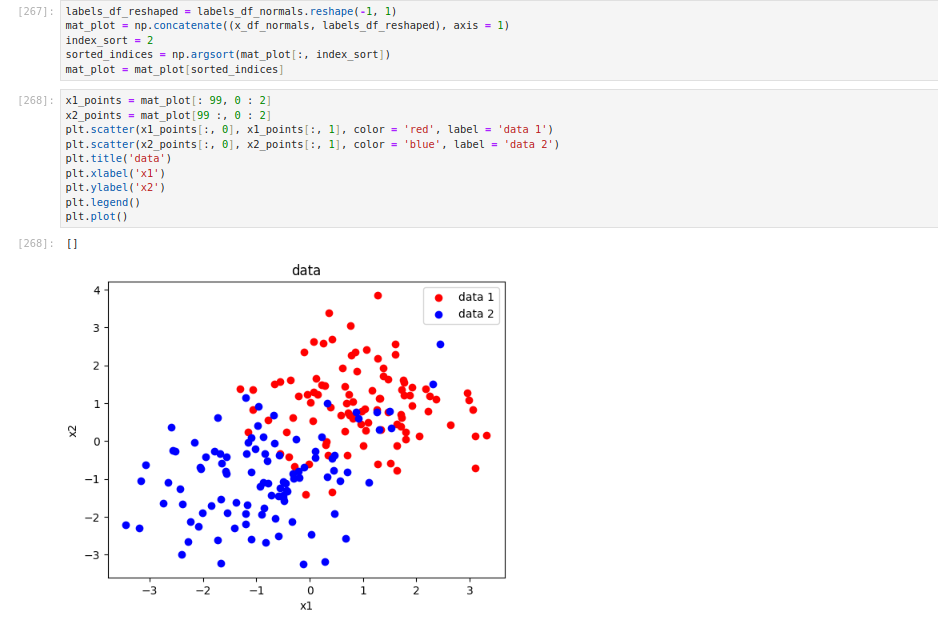
\includegraphics[height=2in]{exercise_pic/normals/plot_data_normals.png}

\end{center}
Inicialmente foi utilizado uma ELM com apenas 5 neurônios na camada intermediária. A matriz de confusão e o gráfico de separação mostram que a expansão aleatória com 5 neurônios está separando bem o modelo e não gerando overfitting.

\begin{center}

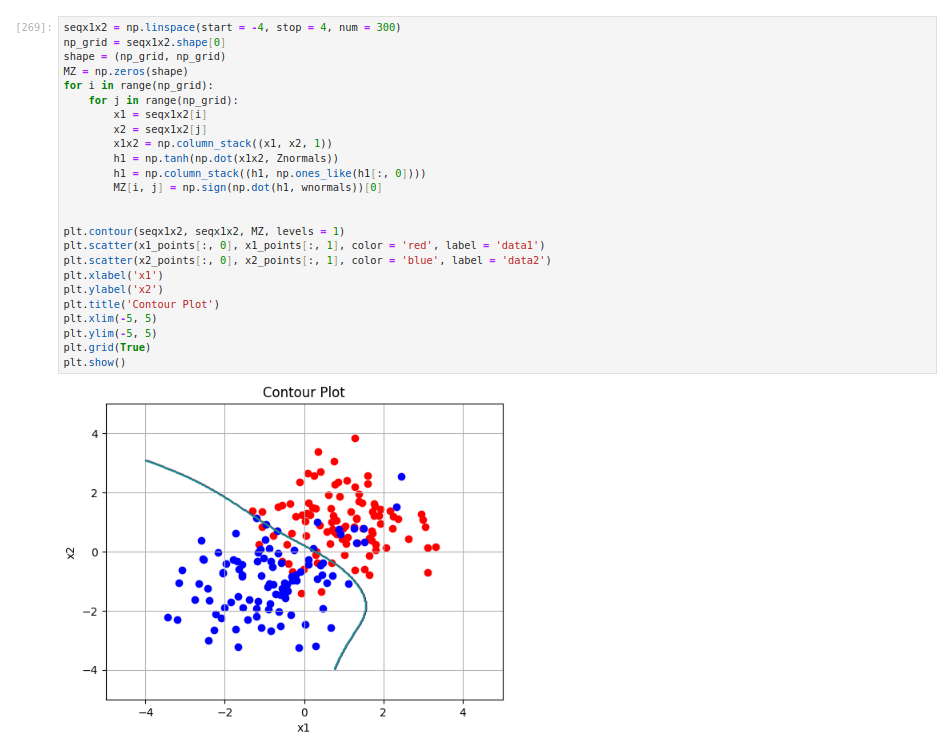
\includegraphics[height=3in]{exercise_pic/normals/sep_plot_normals5.png}
\vspace{10pt}

\end{center}

\begin{center}

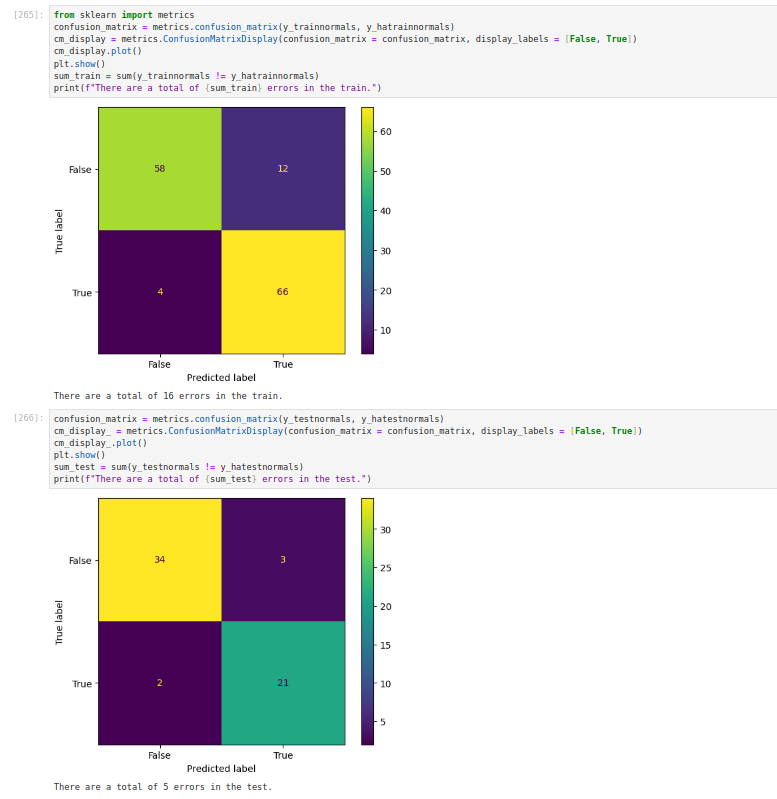
\includegraphics[height=3in]{exercise_pic/normals/conf_matrix_normals5.png}
\vspace{10pt}
    
\end{center}
Usando 10 neurônios na camada intermediária, podemos perceber uma tendência não linear de separação no gráfico dos dados.

\begin{center}

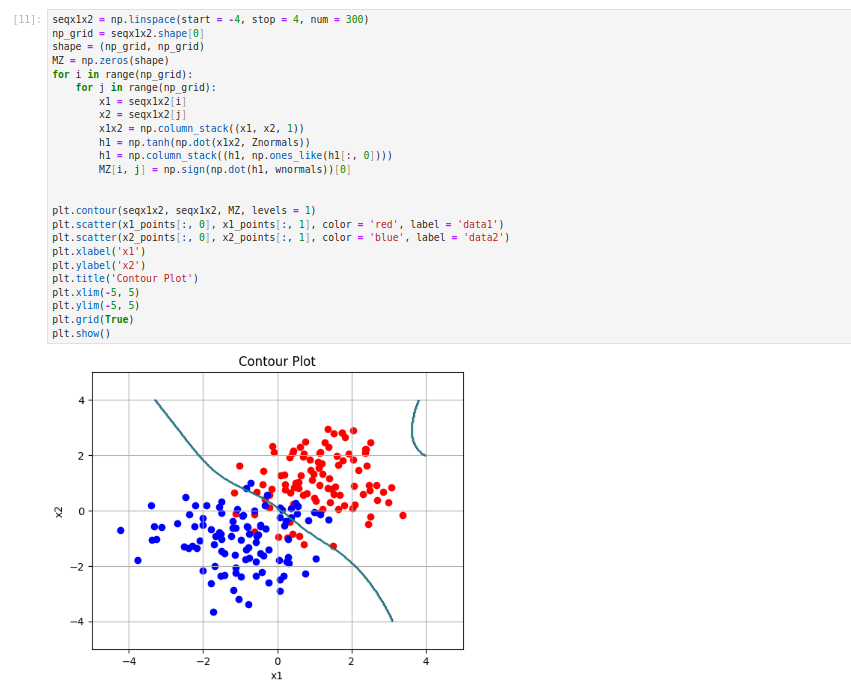
\includegraphics[height=3in]{exercise_pic/normals/plot_data_normals_10.png}
\vspace{10pt}

\end{center}

\begin{center}

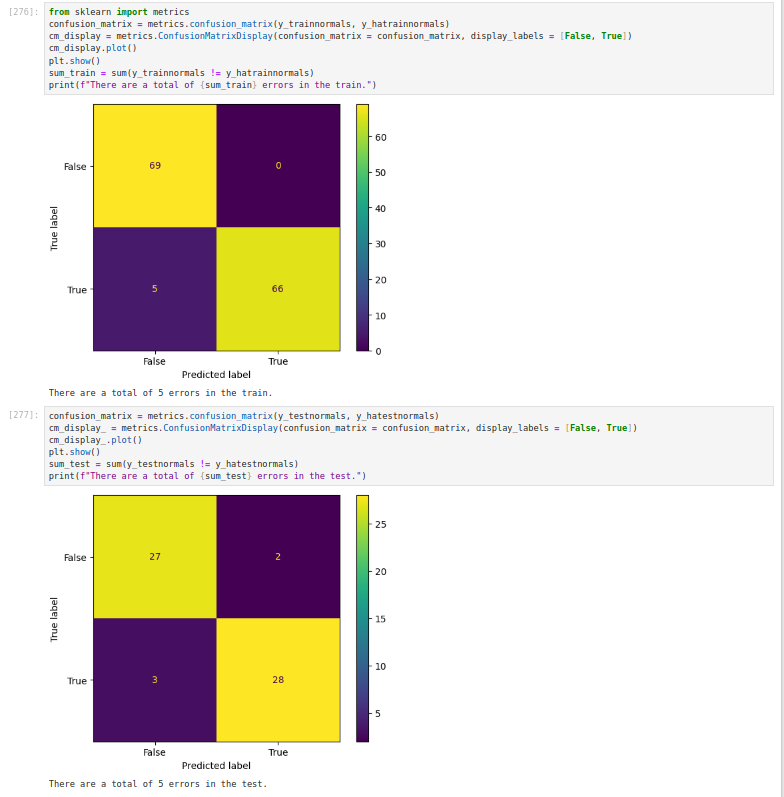
\includegraphics[height=3in]{exercise_pic/normals/conf_matrix_normals10.png}
\vspace{10pt}
    
\end{center}
Usando 30 neurônios na camada intermediária, é possível observar claramente uma boa separação dos dados, no gráfico de separação. No entanto, deve-se tomar cuidado para não colocar muitos neurônios na camada intermediária, gerar um modelo com overfitting e não conseguir generalizar uma boa saída para novos dados, diferentes dos de treinamento.

\begin{center}

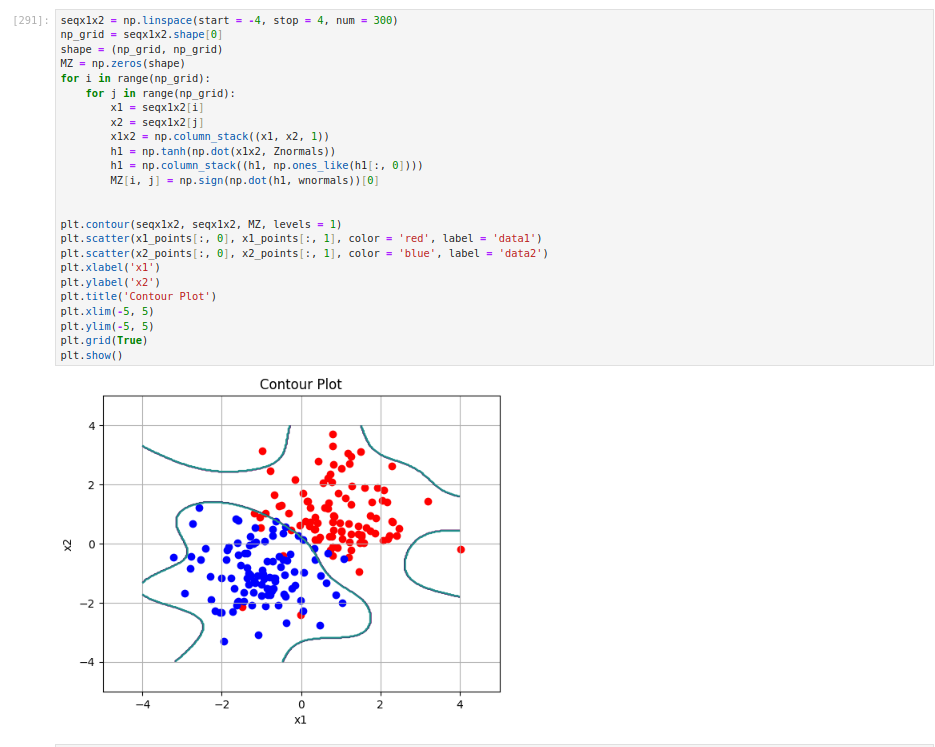
\includegraphics[height=3in]{exercise_pic/normals/sep_plot_normals30.png}
\vspace{10pt}

\end{center}


\begin{center}

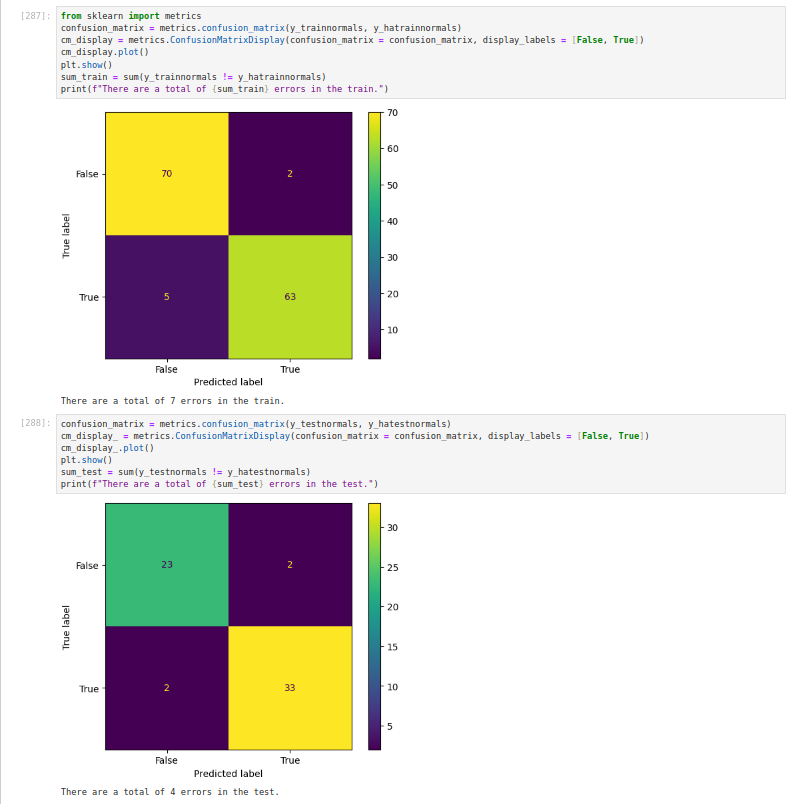
\includegraphics[height=3in]{exercise_pic/normals/conf_matrix_normals30.png}
\vspace{10pt}
    
\end{center}
Portanto, utilizando o modelo com apenas 6 neurônios na camada intermediária aparenta uma boa aproximação sem tendência a overfitting. A imagem abaixo mostra a separação utilizando 6 neuronios na camada intermediaria : 

\begin{center}

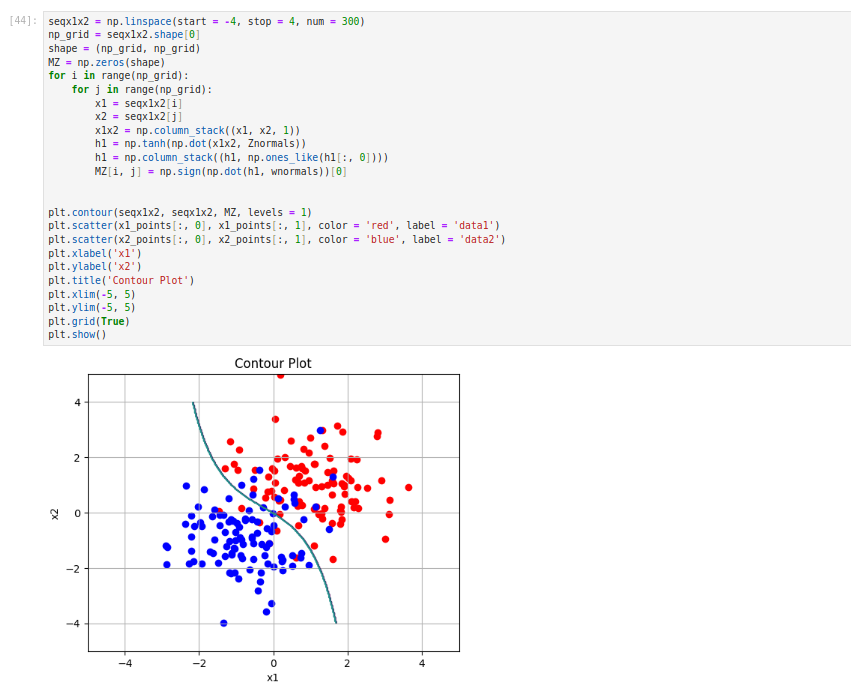
\includegraphics[height=3in]{exercise_pic/normals/plot_6_neurons.png}
\vspace{10pt}
    
\end{center}









\subsection{xor}


O segundo problema terá seus dados gerados também pelo pacote mlbench e são retratados abaixo : 

\begin{center}

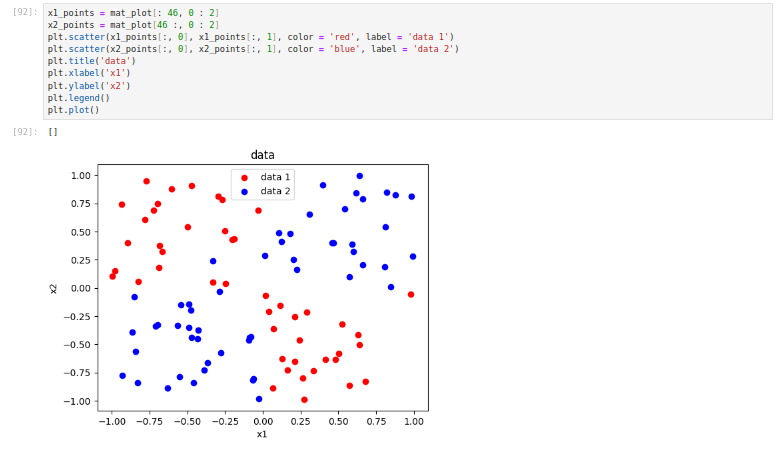
\includegraphics[height=2in]{exercise_pic/xor/plot_data_xor.png}

\end{center}
\vspace{5pt}
Inicialmente foi utilizado uma ELM com 5 neurônios na camada intermediária. Com apenas 5 neurônios na camada intermediária, é possível concluir que o modelo obteve um alto erro para os dados tanto de treino quanto de teste. A matriz de confusão e o gráfico de separação estão plotados abaixo :

\begin{center}

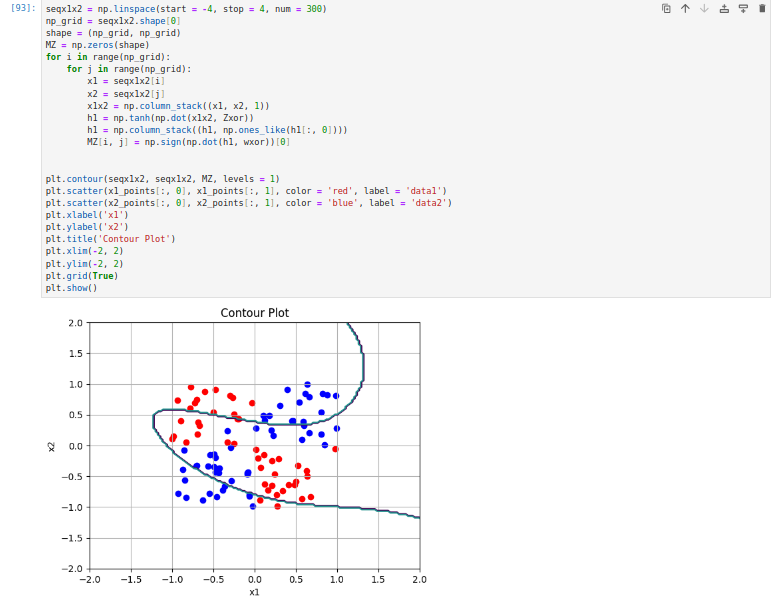
\includegraphics[height=3in]{exercise_pic/xor/plot_graph_xor_5.png}
\vspace{10pt}

\end{center}


\begin{center}

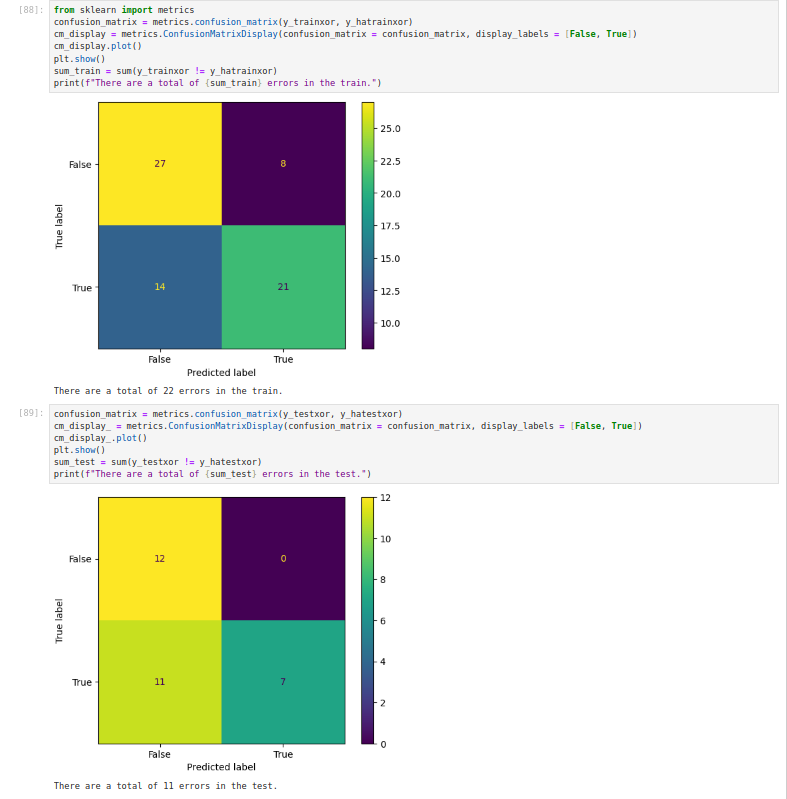
\includegraphics[height=3in]{exercise_pic/xor/conf_matrix_5_xor.png}
\vspace{10pt}
    
\end{center}
Usando 10 neurônios na camada intermediária, podemos observar ainda uma boa separação e um menor erro para os dados de teste.

\begin{center}

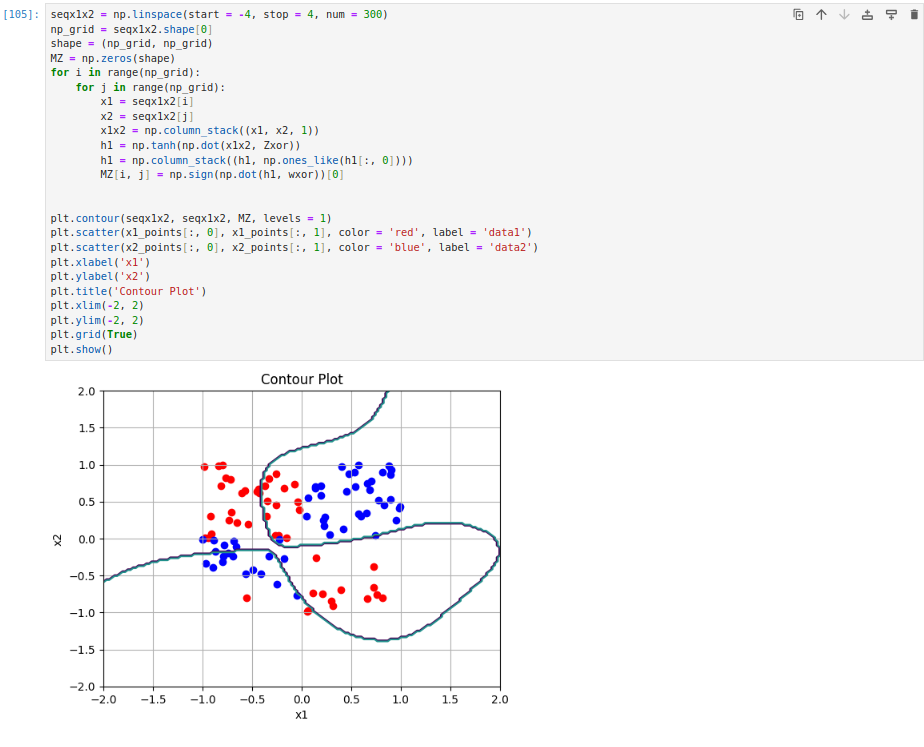
\includegraphics[height=3in]{exercise_pic/xor/plot_graph_xor_10.png}
\vspace{10pt}

\end{center}


\begin{center}

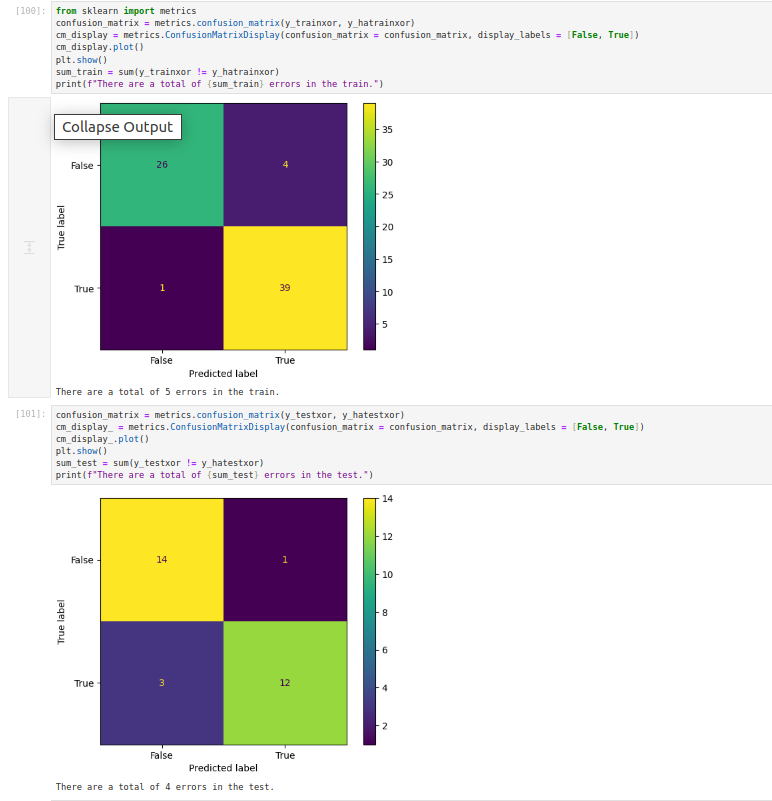
\includegraphics[height=3in]{exercise_pic/xor/conf_matrix_10_xor.png}
\vspace{10pt}
    
\end{center}
Usando 30 neurônios na camada intermediária, é possível concluir que há um overfitting do modelo.

\begin{center}

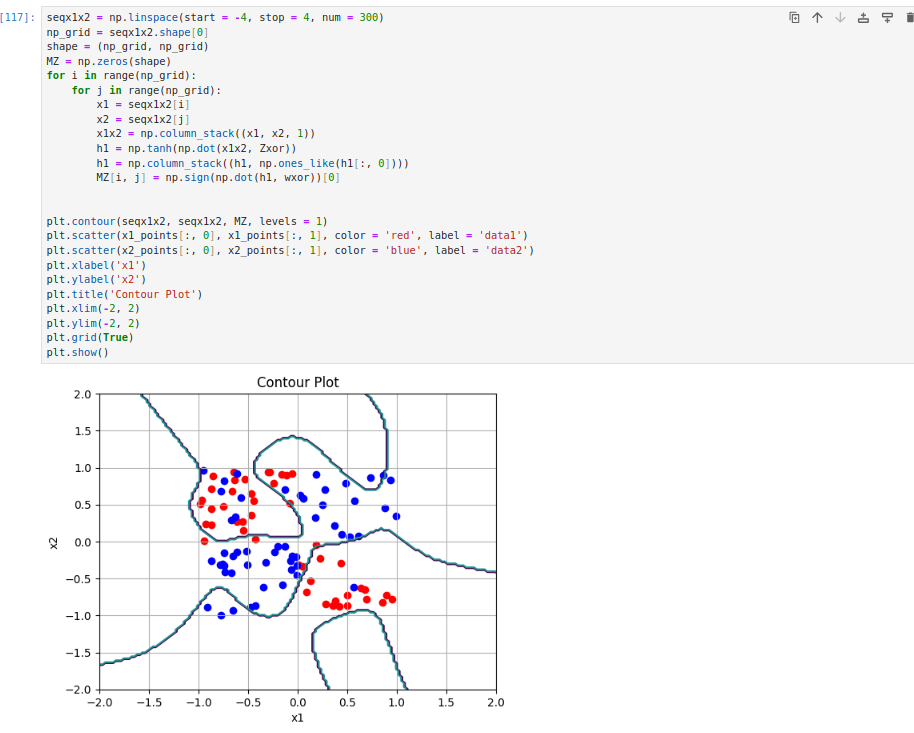
\includegraphics[height=3in]{exercise_pic/xor/plot_graph_xor_30.png}
\vspace{10pt}

\end{center}


\begin{center}

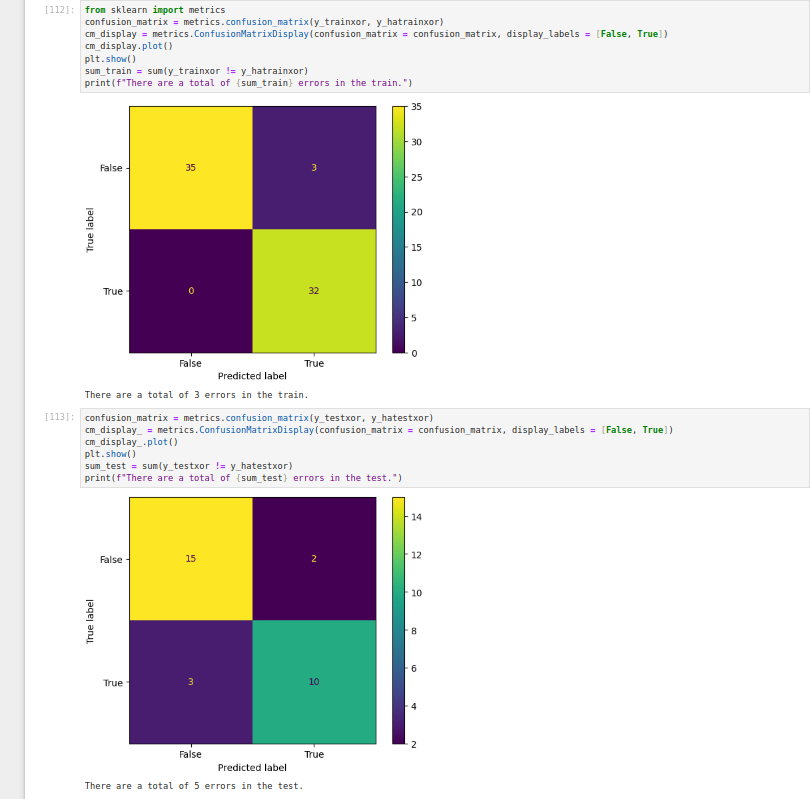
\includegraphics[height=3in]{exercise_pic/xor/conf_matrix_30_xor.png}
\vspace{10pt} 

Portanto, podemos concluir que o modelo com 10 neuronios na camada intermediaria gerará uma boa saída para os dados de entrada.

\end{center}






\subsection{circle}


O terceiro problema terá seus dados gerados também pelo pacote mlbench e são retratados abaixo : 

\begin{center}

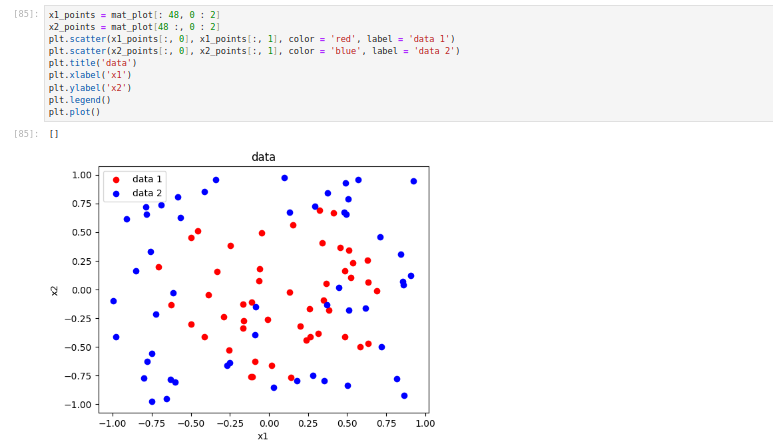
\includegraphics[height=2in]{exercise_pic/circle/data_circle.png}

\end{center}
\vspace{5pt}
Com apenas 5 neurônios na camada intermediária, é possível concluir que o modelo obteve um alto erro para os dados tanto de treino quanto de teste. A matriz de confusão e o gráfico de separação estão plotados abaixo :

\begin{center}

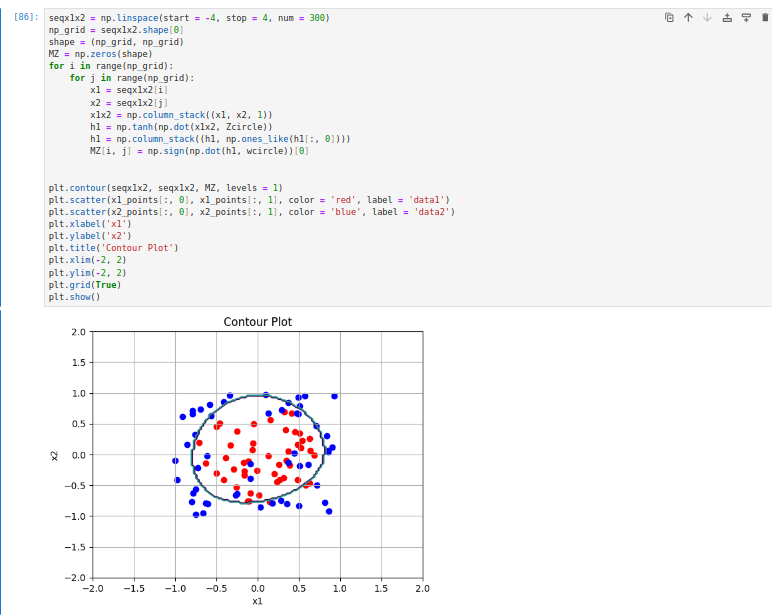
\includegraphics[height=3in]{exercise_pic/circle/plot_graph_circle_5.png}
\vspace{10pt}

\end{center}


\begin{center}

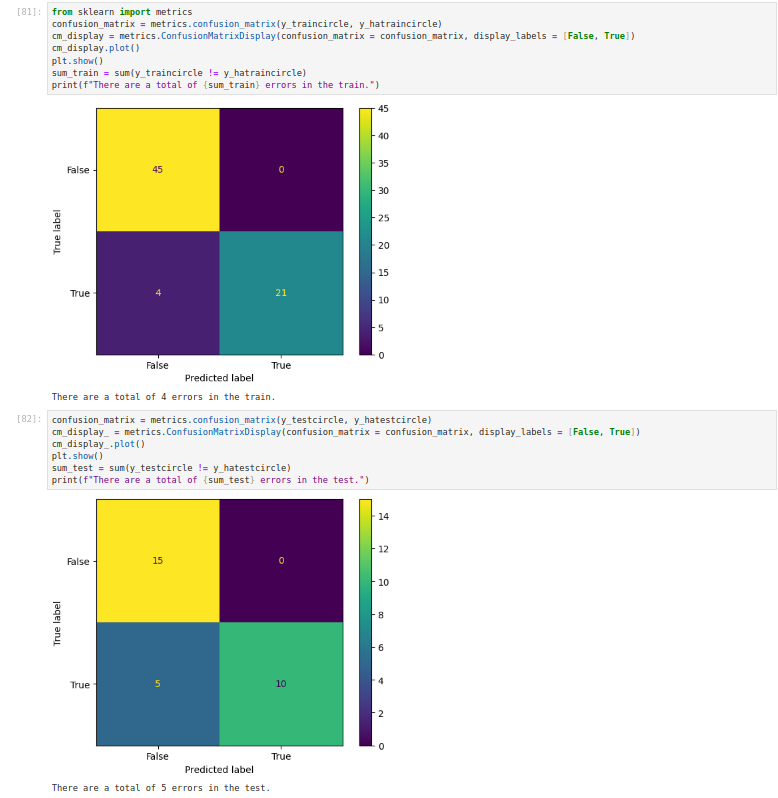
\includegraphics[height=3in]{exercise_pic/circle/conf_matrix_circle_5.png}
\vspace{10pt}
    
\end{center}
Usando 10 neurônios na camada intermediária, podemos observar ainda uma boa separação e um menor erro para os dados de teste.

\begin{center}

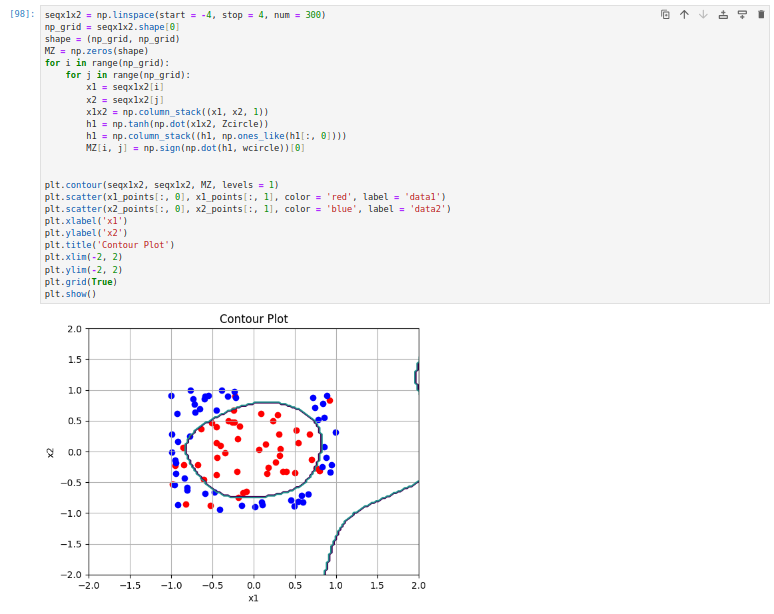
\includegraphics[height=3in]{exercise_pic/circle/plot_graph_10.png}
\vspace{10pt}

\end{center}


\begin{center}

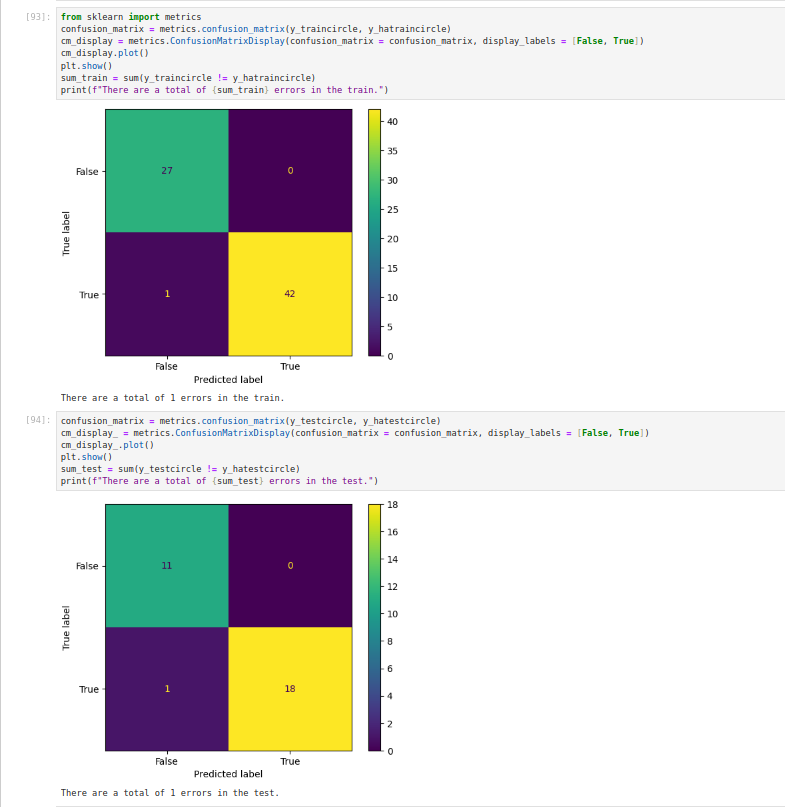
\includegraphics[height=3in]{exercise_pic/circle/conf_matrix_10.png}
\vspace{10pt}
    
\end{center}
Usando 30 neurônios na camada intermediária, é possível concluir que há um overfitting do modelo.

\begin{center}

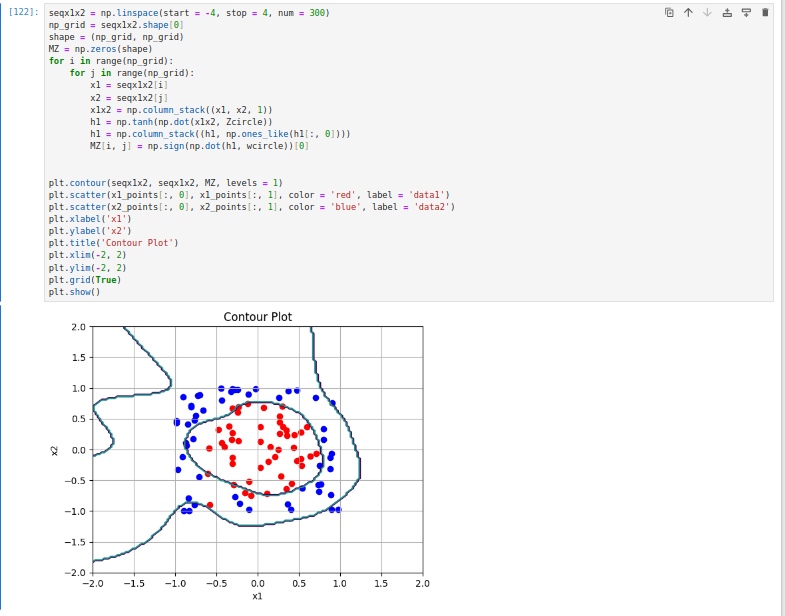
\includegraphics[height=3in]{exercise_pic/circle/plot_graph_30.png}
\vspace{10pt}

\end{center}


\begin{center}

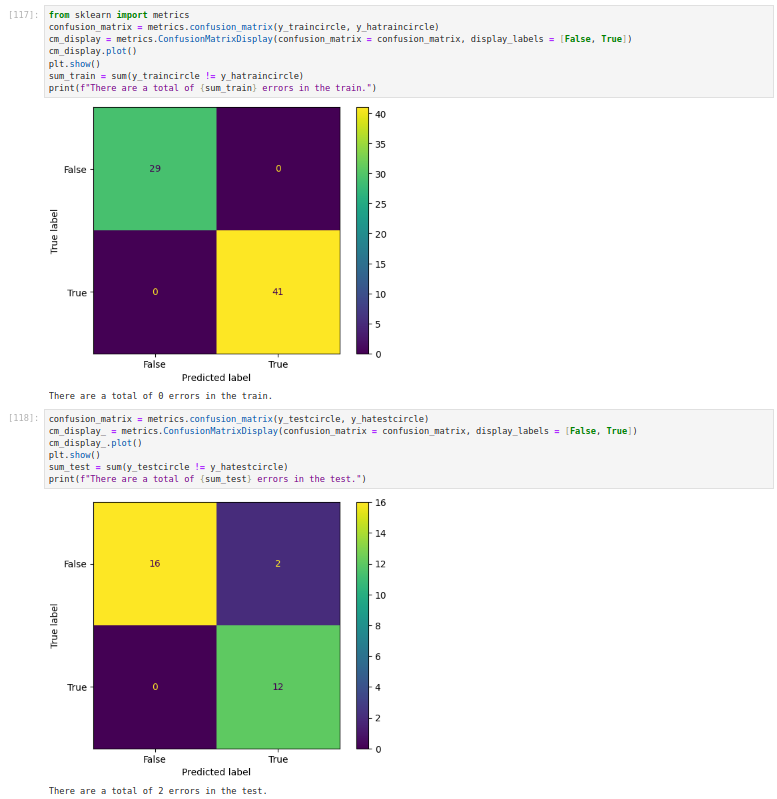
\includegraphics[height=3in]{exercise_pic/circle/conf_matrix_30.png}
\vspace{10pt} 

Portanto, podemos concluir que o modelo com 10 neuronios na camada intermediaria gerará uma boa saída para os dados de entrada.

\end{center}





























\subsection{spirals}


O último problema terá seus dados gerados também pelo pacote mlbench, contém um formato espiral e são retratados abaixo : 

\begin{center}

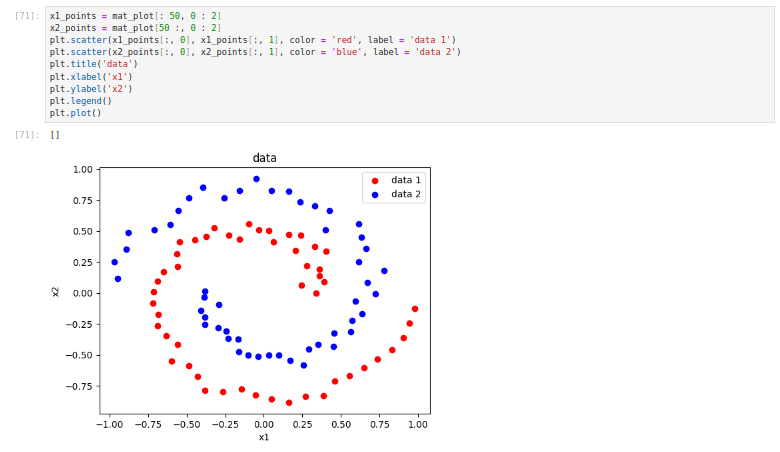
\includegraphics[height=2in]{exercise_pic/spirals/plot_graph_spirals.png}

\end{center}
\vspace{5pt}
Inicialmente foi utilizado uma ELM com 5 neurônios na camada intermediária. Com apenas 5 neurônios na camada intermediária, é possível concluir que o modelo obteve um alto erro para os dados tanto de treino quanto de teste, os erros foram bastante altos e podemos considerar isso como um underfitting. A matriz de confusão e o gráfico de separação estão plotados abaixo :

\begin{center}

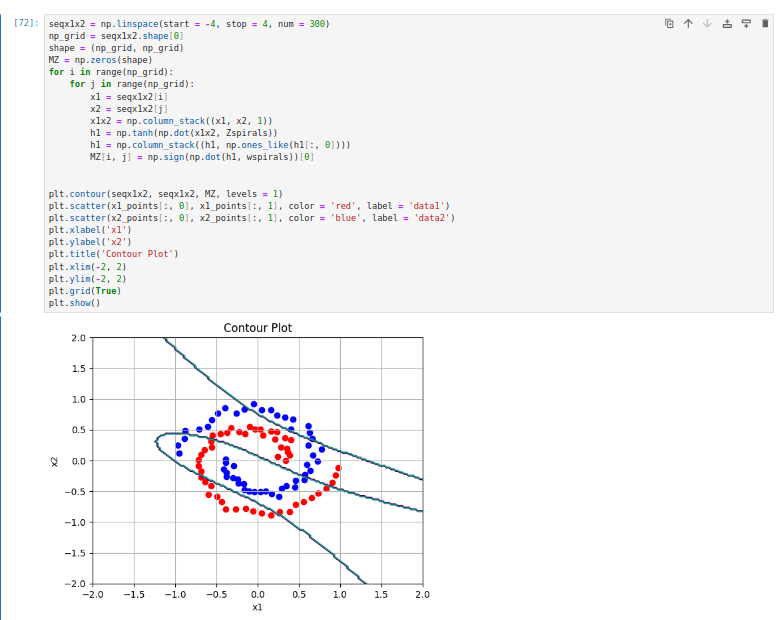
\includegraphics[height=3in]{exercise_pic/spirals/plot_graph_sep_spirals_5.png}
\vspace{10pt}

\end{center}


\begin{center}

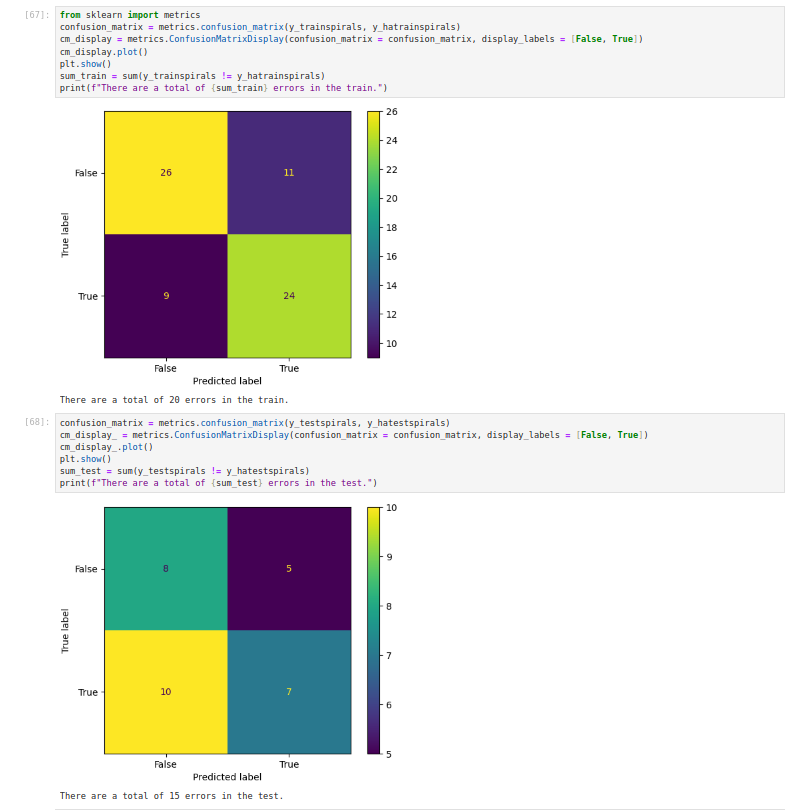
\includegraphics[height=3in]{exercise_pic/spirals/conf_matrix_spirals_5.png}
\vspace{10pt}
    
\end{center}
Usando 10 neurônios na camada intermediária, podemos observar ainda uma boa separação e um menor erro para os dados de teste.

\begin{center}

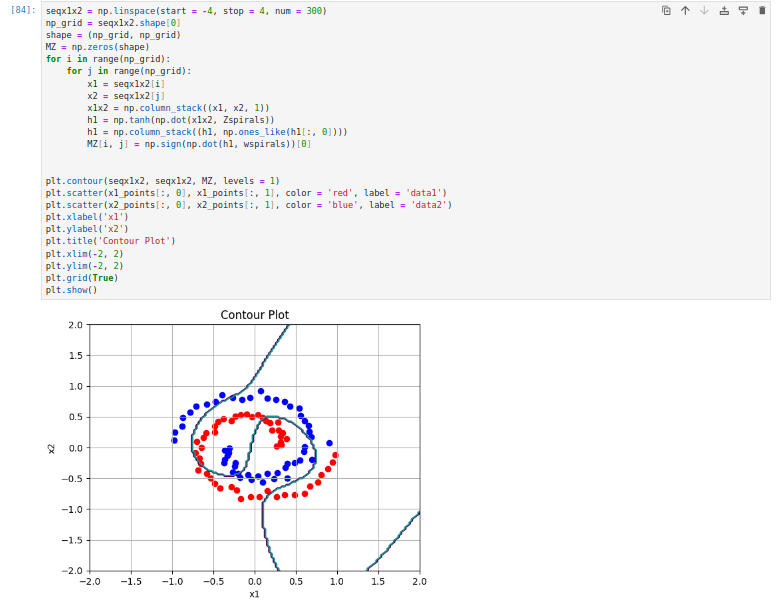
\includegraphics[height=3in]{exercise_pic/spirals/plot_graph_sep_spirals_10.png}
\vspace{10pt}

\end{center}


\begin{center}

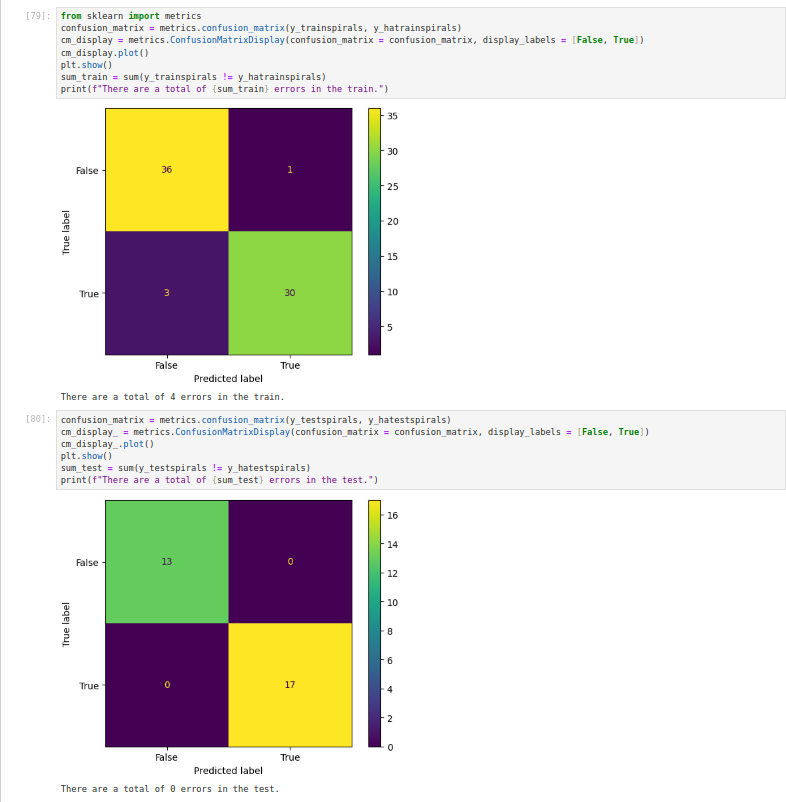
\includegraphics[height=3in]{exercise_pic/spirals/conf_matrix_spirals_10.png}
\vspace{10pt}
    
\end{center}
Usando 30 neurônios na camada intermediária, é possível concluir que há um overfitting do modelo.

\begin{center}

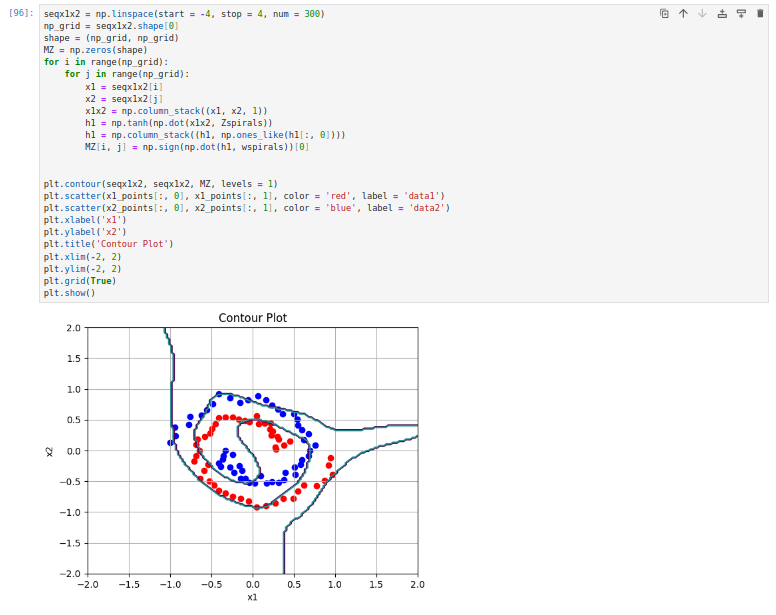
\includegraphics[height=3in]{exercise_pic/spirals/plot_graph_sep_spirals_30.png}
\vspace{10pt}

\end{center}


\begin{center}

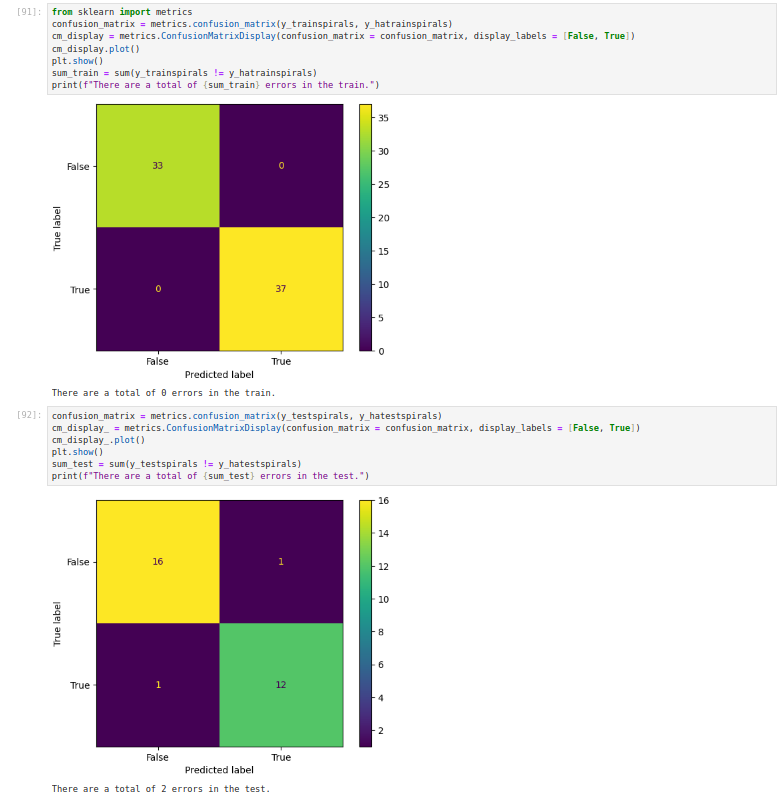
\includegraphics[height=3in]{exercise_pic/spirals/conf_matrix_spirals_30.png}
\vspace{10pt} 

Portanto, podemos concluir que o modelo com 10 neuronios na camada intermediaria gerará uma boa saída para os dados de entrada. Para observar o resultado, basta analisar a matriz de confusão dos dados de teste ao usar 10 neuronios na camada intermediária. O erro sobre os dados de teste foi 0 e portanto o modelo generalizou bem a função geradora.

\end{center}










\end{document}